\chapter{Introduction}
\label{chapter1}


In language learning, the right usage of vocabularies is very important for non-native speakers when they learn a second language. It is necessary to find out the errors the learners made to help them master a new language. Besides, the automatic grammatical error correction (GEC) system can be needed when people write long documents because people can get bored and ignore many grammatical errors after a long period of work. From these scenarios, we can see that automatic grammatical error correction systems have many potential applications in people’s daily lives. In a word, there is a raising and dramatic request for natural language processing (NLP) techniques which can automatically detect and correct the errors of grammar and word usage which the learners make when they are learning second, or even third languages \cite{leacock2010automated}. To overcome this need, NLP researchers and developers have made a lot of progress in recent years, e.g., the language model, construction of datasets and deep learning techniques, which will be discussed in detail in the literature review.
In recent years, deep learning techniques have shown great power for computer vision and natural language processing \cite{lecun2015deep}. Deep learning techniques are widely used from search engines to recommendation systems in many e-co websites to spam content filtering on social networks with the smartphone playing a more important role in people’s daily life. What’s more, the number of new applications of deep learning is still raising sharply. 

\begin{figure}[ht]
    \centering
    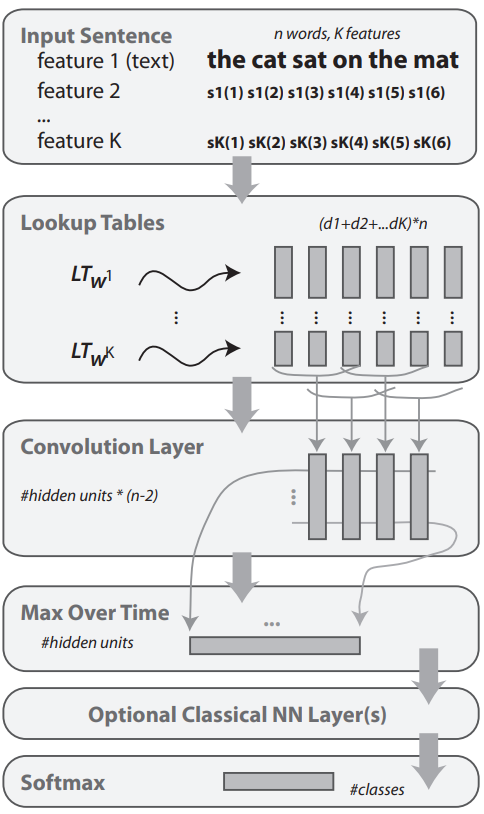
\includegraphics[width=0.5\textwidth]{GDNNNLP.png}
    \caption{A general deep NN architecture for NLP.}
    \label{fig:1}
\end{figure}

In a major part of the research history of NLP, the main methods people apply for NLP problems uses machine learning methods, such as support vector machine (SVM), logistic regression (LR) and shallow neural networks, or even manually designed mechanism with complex rules \cite{young2018recent}. However, these traditional NLP methods run into many problems and can have poor performance. For example, the curse of dimensionality is often met because the representation of language information is often sparse, which leads to a high-dimensional feature expression. What’s more, the traditional NLP methods often depend heavily on manual design, where people often spend a lot of time on writing complex rules. Even though the designers consume so much time on the logical rule design, the mechanism is often incomplete for the fact that the information of human language may change according to different scenarios.

Beside the success of deep learning techniques in computer vision, deep learning also helps to make great progress on NLP with far better performance compared with the traditional NLP methods. A general deep neural network model is shown in Figure~\ref{fig:1}. \cite{collobert2011natural} used a trivial deep learning model to solve NLP problems. The new mechanism at that time outperformed many state-of-art methods, which showed the potential power of deep learning in NLP field. After that time, numerous deep learning NLP methods have been proposed to solve different NLP problem and achieve great success in the different field. The main deep learning applied in NLP includes convolutional neural networks (CNNs), recurrent neural networks (RNNs) and recursive neural networks, which will be explained in detail in later sections.

Applying NLP method to do automatic grammatical error detection and correction is a promising and hot researching area in recent years. A lot of new algorithms and scheme have been proposed to achieve better grammatical error detection and correction. In a word, researchers have done plenty works, which maintain language models, algorithms and dataset. Conll and JFLEG \cite{ng2014conll,napoles2017jfleg} are two famous datasets for the grammatical error correction task. \cite{chollampatt2018multilayer} propose a multilayer convolutional encoder-decoder neural network for grammatical error correction. As the previous neural network model for GEC is time consuming (as it usually takes about several even more than ten days to train a model), \cite{junczys2018approaching} proposal a low resource cost neural networks for GEC task. The works for dataset and neural network model approach will be discussed in detail in the later sections.


\section{Scope}

This project applied the knowledge of deep learning (neural networks), natural language processing, algorithms analysis and basic programming skills. The time spanned from the middle of June to the end of August. The total time period is 11 weeks, of which 2 weeks is spent on literature review, 6 weeks is spent on code implementation and 3 weeks is for the final report. This project is used to detect the grammatical errors made by the beginners of English learning and correct these detected errors into right formats, which has potential applications in many language learning website and mobile applications.

\section{Rationale}
The machine automatic grammatical error correction is a classical researching problem in NLP field. Because of the lack of corpus dataset, the ability of the machine automatic GEC can reach a human-level performance for quite a long time. The new progress on GEC in NLP has been made by applying deep learning techniques. Besides the academic progress, there are many needs in e-co project and smart language teaching. For example, writing is an important part of English learning for non-native speakers and there are large require for detecting and correcting the grammar errors. For the English learners who prepare for English test, e.g., TOFEL or GRE, it would be a large expense if every training passage is commented manually. For the need of grammatical error detection and correction in people’s daily life, this project attempts to build an automatic grammatical error correction system by applying the new techniques of deep learning.

\section{Objective}
The aim of this project is to investigate neural network techniques in NLP for automatic grammatical error correction for writing checking, correction and evaluation applications. First of all, this project constructs a data set which can be used as the training dataset and test dataset for training and testing the deep neural network model in the later steps. Due to the limitation of datasets for grammatical error correction, the famous dataset Conll 2013 and JFLEG are usually perform as test data to evaluate the built GEC system and are difficult to get access. We apply artificial error generation techniques for grammatical error correction proposed by \cite{felice2014generating}. We build a sequence-to-sequence model using long short-term memory (LSTM) encoders and decoders with an attention mechanism as described in \cite{bahdanau2014neural} using stochastic gradient descent. Then, we train the built model based on the previously generated training dataset. Finally, we evaluate the performance of the automatic GEC system using real cases. The focus of this project was on deep learning techniques of NLP on the GEC system which combined grammatical error detection and correction.

\section{Methodology}
\begin{itemize}
    \item Review the context of the application: automatic GEC system for passage evolution. In short, the automatic GEC system should detection the grammatical errors in the test sentence and correct the grammatical errors into the right form. This section will mostly focus on the famous dataset for GEC and well-known works of applying deep learning method for GEC tasks.
    \item 	Review of the pivot of research subject: Seq2seq model with LSTM construction. This neural network model consists of two components, the first of which encodes a source sentence $\mathbf{x}$ and the second $\mathbf{y}$. \cite{sutskever2014sequence} said that RNNs with long short term memory (LSTM) units can achieve close to the state-of-the-art performance of the conventional phrase-based machine translation system. This project will combine the above two models and realize this model by programming.
\end{itemize}